\documentclass[18pt, twoside, a4paper, dvipdfm]{book}

\usepackage{hcypaperstyle}

\begin{document}

\title{毕业设计论文}
%\subtitle{插件的加载和初始化}
\author{黄丛宇\\06161032}
\maketitle

\lfour

\zhabstract 
在高速公路上的实时监控系统中,摄像头对运动车辆的拍摄结果无法直接用于位置识别,需要首先对图像进行处理,运动分割是把序列图像分成语义上具有不同意义的区域,进而分割出运动物体的过程,它是许多运动图像分析应用中必不可少的初始处理阶段,在气象、交通和军事等方面有着巨大的应用前景。
本论文的主要内容是对实时监控系统中对运动车辆的分割的研究实现,首先介绍了本题目的研究背景与意义,以及作者本人的主要工作,然后简单介绍数字图像基本理论,流程与方法包括运动图像分割的方法,下来对运动车辆分割系统进行分析与设计,接着采用Matlab编程整体结构,利用Matlab的强大图像处理功能与GUIDE 成熟的GUI编程结合,总体采用帧间差分法,抽取背景法与光流法等三种方法来对运动车辆分割系统进行实现并测试,最后对这三种方法进行比较并得出结论。
本系统的输入为经过了图像处理前两步骤的图像预处理与图像恢复之后得到的输出,输出为从图像中分割出的目标图像段。系统成果可直接用于一段交通录像并对其中的车辆进行检测与分割,从而实现对交通的各种监管和事故发生后的责任追究等。本系统的实现,能够辅助交通监管系统进行路段状况分析。
{\zhkeywords 图像处理;图像分割;Matlab;GUIDE;运动图像}

\enabstract
In the supervise system on the freeway, the image that camera take from the cars can not be used immediately in identification of posiiton, it’s need to do some process. Image segmentation is a very important part of image processing, and is widely used in traffic, weather, army and so on. 

This paper is mainly about the research and implement of the image segmentation in the real-time supervise system. It first introduces the background and meaning of this topic and author’s work. Second, it introduce the base digital image processing theories, its work flow and work method. Then System is analysis and designed. Then use Matlab  programming ,with the capability of image-processing toolbox of matlab to work with GUIDE together ,and totally use inter-frame differ, background segmentation and optic flow three methods to implement. At last compare the three methods and gives the conclusion.

The input of this system is the output of pre-processing and image restoration. And output is the target image segment that split from the input image .The System can immediately used with a input of a piece of video ,recognize and segment the cars in the video ,so we can supervise the traffic condition and go behind someone before an accident and so on. This system can do some help in traffic surveillance and control.

{\enkeywords image processing;image segmentation;Matlab;GUIDE;Movement image}

\newpage
\tableofcontents

\chapter{绪论}
\section{研究背景和意义}
\subsection{图像处理背景}
1.图像是人类获取和交换信息的主要来源,因此,图像处理的应用领域必然涉及到人类生活和工作的方方面面。随着人类活动范围的不断扩大,图像处理的应用领域也将随之不断扩大:
2.航天和航空技术方面的应用:数字图像处理技术在航天和航空技术方面的应用,除了JPL对月球、火星照片的处理之外,在飞机遥感和卫星遥感技术中也有很多应用。许多国家每天派出很多侦察飞机对地球上有兴趣的地区进行大量的空中摄影。对由此得来的照片进行处理分析,以前需要雇用几千人,而现在改用配备有高级计算机的图像处理系统来判读分析,既节省人力,又加快了速度,还可以从照片中提取人工所不能发现的大量有用情报。从60年代末以来,美国及一些国际组织发射了资源遥感卫星(如LANDSAT系列)和天空实验室(如SKYLAB),由于成像条件受飞行器位置、姿态、环境条件等影响,图像质量总不是很高。因此,以如此昂贵的代价进行简单直观的判读来获取图像是不合算的,而必须采用数字图像处理技术。如LANDSAT系列陆地卫星,采用多波段扫描器(MSS),在900km高空对地球每一个地区以18天为一周期进行扫描成像,其图像分辨率大致相当于地面上十几米或100米左右(如1983年发射的LANDSAT-4,分辨率为30m)。这些图像在空中先处理(数字化,编码)成数字信号存入磁带中,在卫星经过地面站上空时,再高速传送下来,然后由处理中心分析判读。这些图像无论是在成像、存储、传输过程中,还是在判读分析中,都必须采用很多数字图像处理方法。现在世界各国都在利用陆地卫星所获取的图像进行资源调查(如森林调查、海洋泥沙和渔业调查、水资源调查等),灾害检测(如病虫害检测、水火检测、环境污染检测等),资源勘察(如石油勘查、矿产量探测、大型工程地理位置勘探分析等),农业规划(如土壤营养、水份和农作物生长、产量的估算等),城市规划(如地质结构、水源及环境分析等)。我国也陆续开展了以上诸方面的一些实际应用,并获得了良好的效果。在气象预报和对太空其它星球研究方面,数字图像处理技术也发挥了相当大的作用。 

\begin{figure}[htbp]
\centering
\setlength{\abovecaptionskip}{0pt} 
\setlength{\belowcaptionskip}{10pt} 
\caption{测试图片}
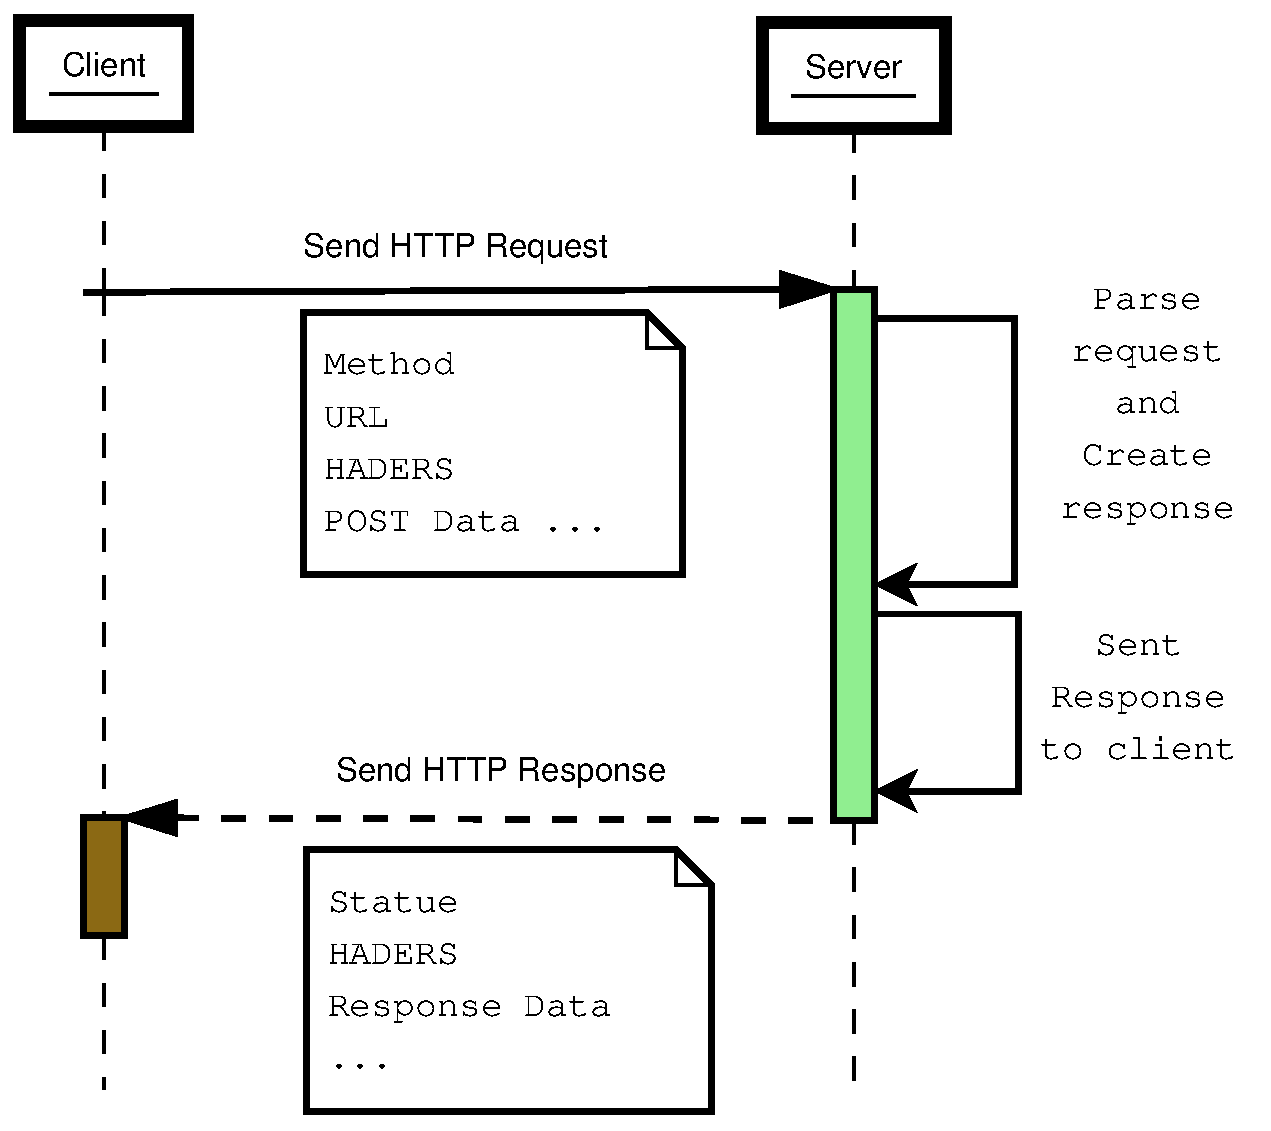
\includegraphics[height=6cm, width=10cm]{http.eps}
\end{figure}

3.生物医学工程方面的应用:数字图像处理在生物医学工程方面的应用十分广泛,而且很有成效。除了CT技术之外,还有一类是对医用显微图像的处理分析,如红单元、白单元分类,染色体分析,癌单元识别等。此外,在X光肺部图像增晰、超声波图像处理、心电图分析、立体定向放射治疗等医学诊断方面都广泛地应用图像处理技术。 
4.通信工程方面的应用:当前通信的主要发展方向是声音、文字、图像和数据结合的多媒体通信。具体地讲是将电话、电视和计算机以三网合一的方式在数字通信网上传输。其中以图像通信最为复杂和困难,因图像的数据量十分巨大,如传送彩色电视信号的速率达100Mbit/s以上。要将这样高速率的数据实时传送出去,必须采用编码技术来压缩信息的比特量。在一定意义上讲,编码压缩是这些技术成败的关键。除了已应用较广泛的熵编码、DPCM编码、变换编码外,目前国内外正在大力开发研究新的编码方法,如分行编码、自适应网络编码、小波变换图像压缩编码等。
5.工业和工程方面的应用:在工业和工程领域中图像处理技术有着广泛的应用,如自动装配线中检测零件的质量、并对零件进行分类,印刷电路板疵病检查,弹性力学照片的应力分析,流体力学图片的阻力和升力分析,邮政信件的自动分拣,在一些有毒、放射性环境内识别工件及物体的形状和排列状态,先进的设计和制造技术中采用工业视觉等等。其中值得一提的是研制具备视觉、听觉和触觉功能的智能机器人,将会给工农业生产带来新的激励,目前已在工业生产中的喷漆、焊接、装配中得到有效的利用。 
6.军事公安方面的应用:在军事方面图像处理和识别主要用于导弹的精确末制导,各种侦察照片的判读,具有图像传输、存储和显示的军事自动化指挥系统,飞机、坦克和军舰模拟训练系统等;公安业务图片的判读分析,指纹识别,人脸鉴别,不完整图片的复原,以及交通监控、事故分析等。目前已投入运行的高速公路不停车自动收费系统中的车辆和车牌的自动识别都是图像处理技术成功应用的例子。 

\begin{table}[htbp]
\setlength{\abovecaptionskip}{0pt} 
\setlength{\belowcaptionskip}{10pt} 
\caption{表格测试}
\centering
\begin{tabularx}{\textwidth}{XXXXl} %最后一列是空的。这样可以是倒数第二列居中,否则会报错或不居中。
\toprule
\centering 名称 & \centering  模块1 & \centering  模块2 &\centering 模块3&\\
\midrule
\centering PLUGIN\_FUNC\_UNSET &\centering  p1 &\centering  p2 &\centering  p3&\\
\centering PLUGIN\_URI\_CLEAN &\centering  p1 &\centering  p2 &\centering  p3&\\
\bottomrule
\end{tabularx}
\end{table}

7.文化艺术方面的应用:目前这类应用有电视画面的数字编辑,动画的制作,电子图像游戏,纺织工艺品设计,服装设计与制作,发型设计,文物资料照片的复制和修复,运动员动作分析和评分等等,现在已逐渐形成一门新的艺术--计算机美术。
在高速公路上的实时监控系统中,摄像头对运动车辆的拍摄结果无法直接用于位置识别,首先需要进行图像分割,图像分割就是把图像分成各具特性的区域并提取出感兴趣目标的技术和过程。而运动分割是把序列图像分成语义上具有不同意义的区域,进而分割出运动物体的过程,它是许多运动图像分析应用中必不可少的初始处理阶段,在气象、交通和军事等方面有着巨大的应用前景。本系统的实现,能够辅助交通监管系统进行路段状况分析,通过本课题,培养本科生综合运用所学知识来解决实际问题的能力。

\subsection{视频车辆监控技术背景}

基于视频图像和字符识别技术的视频车辆自动监控系统是目前极具发展潜力的监控系统之一。它与传统的基于磁环路检测器的交通监控系统相比具有如下优势:
1.安装简单灵活,不用进行路面施工。
2.维护简易,系统升级方便。
3.能够检测多种交通流信息,包括车速、饱和度、占有率等,并且可用于视频的电子警察系统。
现今比较成熟的运动图像分割理论主要包括:
1.空间域灰度分割
2.时间域运动分割[8]
空间域灰度分割:首先对静止帧进行灰度分割,然后利用物体的运动信息,对运动状态相同且空间相邻的灰度区域进行融合。
时间域运动分割:主要是利用相邻帧间的相关性,对图像中的像素进行运动估计,根据像素间运动矢量的不同,对图像进行分割。

\section{研究目标及作者的主要工作}
本论文主要阐述基于视频图像技术的视频车辆自动监控系统中图像分割部份的系统实现过程与分割算法比较。主要采用的理论是以时间域为主的运动分割,希望通过使用帧间差分法,抽取背景法与光流法三种方法来实现实时监控系统中运动车辆的分割并对这三种种方法进行比较并得出结论。

主要工作内容:
1.阅读相关资料文献,掌握有关图像处理及图像分割的基础理论知识;
2.编写算法实现对帧序列的截取;
3.使用Matlab函数编程完成对运动车辆的分离;
4.进行可视化的GUIDE GUI编程,实现完整的运动车辆分离系统;
5.系统测试,运行结果展示;
6.比较各种算法优劣,得出结论。
1.3本文章节结构

第1章为绪论,主要对本论文的主要内容进行了概述:
首先是数字图像处理课题的历史背景和研究意义,一方面描述数字图像处理当前的发展概况,已经获得的各种研究成果和应用前景,并提出基于视频图像和字符识别技术的视频车辆自动监控系统时下的流行应用与特点,另一方面给出数字图象处理与视频车辆监控的研究意义。
下来是研究目标及作者的主要工作,一方面描述本论文在数字图象处理与视频车辆监控领域内的研究目标,另一方面给出作者本人在毕业设计期间的主要工作内容。
最后是本文的大体章节结构安排。

第2章为数字图像处理原理,主要对数字图像处理研究领域的基本概念和理论知识进行描述。
首先是数字图象处理的概况,简单介绍了数字图象处理的概念与基本特点和优点。
下来是数字图形处理的方向分类,介绍了数字图象处理时下的主要几个研究方向。
最后是数字图象处理的流程与运算方法,介绍了数字图像处理的四个基础步骤,每个步骤的主要工作内容,以及数字图象处理的8种基本运算方法。

第3章为运动车辆分割系统的分析与设计,首先阐述了运动图像分割的原理,其次是提出运动车辆分割系统的需求分析,功能模块划分,性能分析,运行环境规定等,最后是系统的设计,包括基础设计思路,接口设计与算法流程设计。
第一部分阐述运动图像分割原理,从技术层面上对运动图像分割的原理和方法进行解释和示例。
第二部分为系统分析,对系统流程,功能需求,模块划分,性能与运行环境进行分析。
第三部分为系统设计,重点是接口设计与算法流程设计。

第4章为运动车辆分割系统的实现与测试,为本论文的核心部份
首先是系统实现,分为算法实现与接口实现,算法实现对帧间差分法,抽取背景法,光流法三种方法的优缺点分别进行探讨,并分别用三种方法来对运动车辆的分割进行实现,并列出分割结果。接口实现则主要是使用simulink和callback实现内部接口和使用GUIDE用户接口进行实现,与接口设计相呼应。
然后是系统测试,分为功能测试与性能测试,功能测试根据前面功能需求分析的用例划分,相对地对每个用例进行测试,给出已经修复的BUG与产生BUG的原因和解决方法。并给出测试结果与测试结论。性能测试则主要是从空间和时间两方面上对本系统进行性能测试和评估,以确定其是否达到了预期的性能要求。

第5章为结束语,包括整篇论文的总结与对数字图象处理与视频车辆监控的展望。
首先是总结,包括对本论文的全面概括以及三种算法实现后的结果比较并得出结论,还有作者本人在本次毕业设计中所完成的工作。
然后是展望,对数字图象处理领域的前景作出展望并且提出本运动车辆分割系统的不足和改进期望。

\chapter{数字图像处理技术}
\section{数字图像处理概述}

	数字图像处理(Digital Image Processing)又称为计算机图像处理,它是指将图像信号转换成数字信号并利用计算机对其进行处理的过程。[5]数字图像处理最早出现于20世纪50年代,当时的电子计算机已经发展到一定水平,人们开始利用计算机来处理图形和图像信息。数字图像处理作为一门学科大约形成于20世纪60年代初期。早期的图像处理的目的是改善图像的质量,它以人为对象,以改善人的视觉效果为目的。图像处理中,输入的是质量低的图像,输出的是改善质量后的图像,常用的图像处理方法有图像增强、复原、编码、压缩等。首次获得实际成功应用的是美国喷气推进实验室(JPL)。他们对航天探测器徘徊者7号在1964年发回的几千张月球照片使用了图像处理技术,如几何校正、灰度变换、去除噪声等方法进行处理,并考虑了太阳位置和月球环境的影响,由计算机成功地绘制出月球表面地图,获得了巨大的成功。随后又对探测飞船发回的近十万张照片进行更为复杂的图像处理,以致获得了月球的地形图、彩色图及全景镶嵌图,获得了非凡的成果,为人类登月创举奠定了坚实的基础,也推动了数字图像处理这门学科的诞生。在以后的宇航空间技术,如对火星、土星等星球的探测研究中,数字图像处理技术都发挥了巨大的作用。 数字图像处理取得的另一个巨大成就是在医学上获得的成果。1972年英国EMI公司工程师Housfield发明了用于头颅诊断的X射线计算机断层摄影装置,也就是我们通常所说的CT(Computer Tomograph)。CT的基本方法是根据人的头部截面的投影,经计算机处理来重建截面图像,称为图像重建。1975年EMI公司又成功研制出全身用的CT装置,获得了人体各个部位鲜明清晰的断层图像。1979年,这项无损伤诊断技术获得了诺贝尔奖,说明它对人类作出了划时代的贡献。 与此同时,图像处理技术在许多应用领域受到广泛重视并取得了重大的开拓性成就,属于这些领域的有航空航天、生物医学工程、工业检测、机器人视觉、公安司法、军事制导、文化艺术等,使图像处理成为一门引人注目、前景远大的新型学科。 随着图像处理技术的深入发展,从70年代中期开始,随着计算机技术和人工智能、思维科学研究的迅速发展,数字图像处理向更高、更深层次发展。人们已开始研究如何用计算机系统解释图像,实现类似人类视觉系统理解外部世界,这被称为图像理解或计算机视觉。很多国家,特别是发达国家投入更多的人力、物力到这项研究,取得了不少重要的研究成果。其中代表性的成果是70年代末MIT的Marr提出的视觉计算理论,这个理论成为计算机视觉领域其后十多年的主导思想。图像理解虽然在理论方法研究上已取得不小的进展,但它本身是一个比较难的研究领域,存在不少困难,因人类本身对自己的视觉过程还了解甚少,因此计算机视觉是一个有待人们进一步探索的新领域。

数字图像处理的基本特点:

	(1)目前,数字图像处理的信息大多是二维信息,处理信息量很大。如一幅低分辨率黑白图像,要求约的数据量;对高分辨率彩色图像,则要求768kbit数据量;如果要处理30帧/秒的电视图像序列,则每秒要求t数据量。因此对计算机的计算速度、存储容量等要求较高。 
(2)数字图像处理占用的频带较宽。与语言信息相比,占用的频带要大几个数量级。如电视图像的带宽约5.6MHz,而语音带宽仅为4kHz左右。所以在成像、传输、存储、处理、显示等各个环节的实现上,技术难度较大,成本亦高,这就对频带压缩技术提出了更高的要求。 
(3)数字图像中各个像素是不独立的,其相关性大。在图像画面上,经常有很多像素有相同或接近的灰度。就电视画面而言,同一行中相邻两个像素或相邻两行间的像素,其相关系数可达0.9以上,而相邻两帧之间的相关性比帧内相关性一般说还要大些。因此,图像处理中信息压缩的潜力很大。 
(4)由于图像是三维景物的二维投影,一幅图象本身不具备复现三维景物的全部几何信息的能力,很显然三维景物背后部分信息在二维图像画面上是反映不出来的。因此,要分析和理解三维景物必须作合适的假定或附加新的测量,例如双目图像或多视点图像。在理解三维景物时需要知识导引,这也是人工智能中正在致力解决的知识工程问题。 
(5)数字图像处理后的图像一般是给人观察和评价的,因此受人的因素影响较大。由于人的视觉系统很复杂,受环境条件、视觉性能、人的情绪爱好以及知识状况影响很大,作为图像质量的评价还有待进一步深入的研究。另一方面,计算机视觉是模仿人的视觉,人的感知机理必然影响着计算机视觉的研究。例如,什么是感知的初始基元,基元是如何组成的,局部与全局感知的关系,优先敏感的结构、属性和时间特征等,这些都是心理学和神经心理学正在着力研究的课题。[1]

数字图象处理的优点:

	1. 再现性好 数字图像处理与模拟图像处理的根本不同在于,它不会因图像的存储、传输或复制等一系列变换操作而导致图像质量的退化。只要图像在数字化时准确地表现了原稿,则数字图像处理过程始终能保持图像的再现。 
2.处理精度高 按目前的技术,几乎可将一幅模拟图像数字化为任意大小的二维数组,这主要取决于图像数字化设备的能力。对计算机而言,不论数组大小,也不论每个像素的位数多少,其处理程序几乎是一样的。换言之,从原理上讲不论图像的精度有多高,处理总是能实现的,只要在处理时改变程序中的数组参数就可以了。回想一下图像的模拟处理,为了要把处理精度提高一个数量级,就要大幅度地改进处理装置,这在经济上是极不合算的。 
3.适用面宽 图像可以来自多种信息源,它们可以是可见光图像,也可以是不可见的波谱图像(例如X射线图像、 射线图像、超声波图像或红外图像等)。从图像反映的客观实体尺度看,可以小到电子显微镜图像,大到航空照片、遥感图像甚至天文望远镜图像。这些来自不同信息源的图像只要被变换为数字编码形式后,均是用二维数组表示的灰度图像(彩色图像也是由灰度图像组合成的,例如RGB图像由红、绿、蓝三个灰度图像组合而成)组合而成,因而均可用计算机来处理。即只要针对不同的图像信息源,采取相应的图像信息采集措施,图像的数字处理方法适用于任何一种图像。 
4.灵活性高 图像处理大体上可分为图像的像质改善、图像分析和图像重建三大部分,每一部分均包含丰富的内容。由于图像的光学处理从原理上讲只能进行线性运算,这极大地限制了光学图像处理能实现的目标。而数字图像处理不仅能完成线性运算,而且能实现非线性处理,即凡是可以用数学公式或逻辑关系来表达的一切运算均可用数字图像处理实现。

\section{数字图像处理的方向分类}

图像数字化 通过取样和量化过程将一个以自然形式存在的图像变换为适合计算机处理的数字形式。图像在计算机内部被表示为一个数字矩阵,矩阵中每一元素称为像素。图像数字化需要专门的设备,常见的有各种电子的和光学的扫描设备,还有机电扫描设备和手工操作的数字化仪。 
  图像编码 对图像信息编码,以满足传输和存储的要求。编码能压缩图像的信息量,但图像质量几乎不变。为此,可以采用模拟处理技术,再通过模-数转换得到编码,不过多数是采用数字编码技术。编码方法有对图像逐点进行加工的方法,也有对图像施加某种变换或基于区域、特征进行编码的方法。脉码调制、微分脉码调制、预测码和各种变换都是常用的编码技术。 
  图像增强 使图像清晰或将其转换为更适合人或机器分析的形式。与图像复原不同,图像增强并不要求忠实地反映原始图像。相反,含有某种失真(例如突出轮廓线)的图像可能比无失真的原始图像更为清晰。常用的图像增强方法有:①灰度等级直方图处理:使加工后的图像在某一灰度范围内有更好的对比度;②干扰抑制:通过低通滤波、多图像平均、施行某类空间域算子等处理,抑制叠加在图像上的随机性干扰;③边缘锐化:通过高通滤波、差分运算或某种变换,使图形的轮廓线增强;④伪彩色处理:将黑白图像转换为彩色图像,从而使人们易于分析和检测图像包含的信息。 
  图像复原 除去或减少在获得图像过程中因各种原因产生的退化。这类原因可能是光学系统的像差或离焦、摄像系统与被摄物之间的相对运动、电子或光学系统的噪声和介于摄像系统与被摄像物间的大气湍流等。图像复原常用二种方法。当不知道图像本身的性质时,可以建立退化源的数学模型,然后施行复原算法除去或减少退化源的影响。当有了关于图像本身的先验知识时,可以建立原始图像的模型,然后在观测到的退化图像中通过检测原始图像而复原图像。 
  图像分割 将图像划分为一些互不重叠的区域,每一区域是像素的一个连续集。通常采用把像素分入特定区域的区域法和寻求区域之间边界的境界法。区域法根据被分割对象与背景的对比度进行阈值运算,将对象从背景中分割出来。有时用固定的阈值不能得到满意的分割,可根据局部的对比度调整阈值,这称为自适应阈值。境界法利用各种边缘检测技术,即根据图像边缘处具有很大的梯度值进行检测。这两种方法都可以利用图像的纹理特性实现图像分割。 
图像分析 从图像中抽取某些有用的度量、数据或信息。目的是得到某种数值结果,而不是产生另一个图像。图像分析的内容和模式识别、人工智能的研究领域有交叉,但图像分析与典型的模式识别有所区别。图像分析不限于把图像中的特定区域按固定数目的类别加以分类,它主要是提供关于被分析图像的一种描述。为此,既要利用模式识别技术,又要利用关于图像内容的知识库,即人工智能中关于知识表达方面的内容。图像分析需要用图像分割方法抽取出图像的特征,然后对图像进行符号化的描述。这种描述不仅能对图像中是否存在某一特定对象作出回答,还能对图像内容作出详细描述。
图像特征提取	 通过图像信息去测量,识别或理解其中的对象物,依赖于一些能表征对象物的图像特征,如线,边缘,区域,形状,颜色,纹理等。通过各种处理方法,将包含在图像信息中的必要特征显露出来,并加以量化的处理称之为图像的特征提取。
图像识别与理解 图像识别可以简单地理解为利用提取的图像物特征对事物进行分类处理,如根据颜色特征将新鲜的桃子按成熟度进行分级,按形状特征对杏仁分类等等。所谓图像理解是利用图像信息实现模拟人的视觉系统理解客观事物。如对图像中的田间景物作出解释,成为田间自动作业机的向导。图像识别实际上可看作是一种简单的,仅仅涉及分类的图像理解,而图像理解则是包含更高层次的,达到某些智能化处理的程度。两者之间的关系密切,有时也很难严格区分。图像识别和图像理解已成为在计算机图像处理的几处上发展起来的一门新兴学科。但从广义角度上来看,它们仍然属于图像处理的范畴。
图像存储与检索 为了保存,处理或者传递图像信息,需要将原图像或经过处理的图像信息在计算机中按某种规律存储,必要时可以方便找到它们,即进行图像的检索,这种对图像群体的保管工作是图像处理不可缺少的内容。
图像输入 图像处理的第一步,是获取处理对象的可见模拟图像,并将其转换为计算机能够接受的数字图像,再输入计算机。如果对象物的信息是不可见的,则首先进行所谓的“信息的可视化”或“可见光图像生成”等处理,这样的过程称为图像的输入。
图像输出 用计算机再现输入的,输出的以及中间处理结果的图像内容即称为图像的输出,是人们考察处理结果,获取处理结果所必须的。[5]

\section{数字图像处理的流程与运算方法}
\subsection{数字图象处理的流程}

图像处理(image processing )使用计算机对图像进行一系列加工,以达到所需的结果。常见的处理有图像数字化、图像编码、图像增强、图像复原、图像分割和图像分析等。图像处理一般指数字图像处理。虽然某些处理也可以用光学方法或模拟技术实现,但它们远不及数字图像处理那样灵活和方便,因而数字图像处理成为图像处理的主要方面。
数字图像处理大体上可以分为四个步骤:
图像预处理
图像恢复
图像分割
图像位置识别
由于一般采样到的原始图像会由于拍摄角度,天气,日光等造成各种模糊,噪声等影响图像进行处理的因素,因此首先有必要对原始图像进行预处理。
图像预处理是将图像中感兴趣的特征有选择的突出,而衰减不需要的特征,故改善后的图像不一定要去逼近原图像。
图像恢复也叫图像复原,是图像处理中的一大技术。它需要将图像退化的过程模型化,并根据这个模型采取相反的过程以求得到尽可能接近原始图像的恢复图像。
图像分割,就是按某种策略将图像中的不同区域分割开来,且保证每个区域互不重叠。要保证区域的不重叠,则每块区域应该有明显的特征属性来区别其他区域。图像分割算法就是基于亮度值的两个基本特性:不连续性和相似性。

\subsection{数字图象处理的运算方法}

 数字图像信息可以看成是一个二维数组f(I,j),对它处理的基本过程如同电视光栅扫描过程,按照从左到右,由上到下的顺序进行(图2-1),并在扫描过程中逐点对各像素进行帧处理。这样的扫描过程称为顺向扫描。与此相对的就是由下到上,由右到左的逆向扫描(图2-2),也是一种常见的扫描过程,这种如同光栅扫描的过程仅仅是图像处理中最基本的处理过程。


数字图象处理的基本运算形式:
1.点运算
在对图像各像素进行处理时,只输入该像素本身灰度的运算方式,见公式2-1:

G(I,j) = p(f(I,j))											(2-1)
式中: 
G 	—— 输出图像;
f 	—— 输入图像;
p	—— 转换算法;

2.领域运算
在对图像各像素进行处理时,不仅输入该像素本身灰度,还要输入以该像素为中心的某局部区域(即领域)中的一些像素的灰度进行运算的方式。假设像素f0被f1-f8所包围,那么对于g0 = (f0+f1+f2+..+f8)/9就是一个领域运算。

3.并行运算
并行运算指的是对图像上各像素同时进行相同处理的运算方式。这种运算方式速度快,但只能用于处理结果与处理顺序无关的场合。在点运算处理中,由于各像素的处理与其他像素无关,因此无论采用顺向扫描还是逆向扫描,处理结果是相同的,因此,点运算可以采用并行运算。而领域运算则要分两种情况:若运算所需的算子不是其他像素的处理结果,那么也可以使用并行运算,反之则根据运算顺序的不同会产生不同的结果,不能使用并行运算。

4.串行运算
串行运算是相对并行运算而言的,指的是图像上按照规定的顺序逐个对像素进行处理的运算形式。串行运算中的处理顺序除了上面说的顺向扫描和逆向扫描外还有其他顺序,如边缘跟踪顺序等。这里可以发现,点运算有既可以采用并行运算,也可以采用并行运算的特点。

5.迭代运算
反复多次进行相同处理的运算,称为迭代运算,迭代运算经常用于某些通过一次运算不能达到目的的情况。迭代运算的反复次数可以在处理前设定,也可以在处理过程中根据是否达到处理目的由计算机判别后确定。

6.窗口运算
图像的信息量很大,为减少处理时间,在可能的情况下,常常采用窗口运算来替代全图像运算。所谓窗口运算是指对图像特定的矩形区域进行某种运算的形式。一般,矩形区域由矩形左上角S点的坐标(a,b)和矩形所包含的行数m和列数n确定(图2-3)。矩形区域可以是图像中存在某对象物的位置,也可以是图像中具有代表性特征的区域。
 
图2- 3 窗口运算
7.模板运算
对图像中特定形状的区域进行某种运算的形式称为模板运算。这里的模板就是指特定形状的区域,它常常是与图像中存在的对象物有相同特征的一个局部的子图像。通过对图像上各像素的模板运算,可以找到图像上与模板特征相同的对象物的存在位置。

8.帧运算
以上各种运算都是在一幅图像内进行的,图像与图像之间不发生关系。通常一副完整的图像被称为一帧,在两幅或多幅图像之间进行运算产生一幅新图像的处理称之为帧运算。帧运算可以看成是一种图像合成处理。运算时,将两幅或多幅图像中的对应点用位逻辑运算或算术运算方法进行合成。
合成函数的种类很多,较为简单的比如算术减与异或。[5]

\chapter{运动车辆分割系统的分析与设计}
\section{运动图像分割技术与算法分析}
\subsection{运动图像分割技术}
	
按运动分类,图像可分为静态图像和动态图象。静态图像包括静止图像和凝固图像。每幅图像本身都是一幅静止图像。凝固图像是动态图象中的某一帧。动态图象的快慢以帧率量度,帧率反映了画面运动的连续性。可以看出,动态图象实际上是由一幅幅静态图像按时间排列组成的。
图像分割是从图像处理到图像分析的关键技术。图像分割的种类和方法很多,有些分割算法可直接用于任何图像,而另一些算法只能适用于分割特殊类别的图像。有些算法需要先对图像进行粗分割,因为它们需要从图像中提取出来的信息。没有唯一的标准的方法。分割结果的好坏需要根据具体的场合要求衡量。
早期的图像分割方法可以分为两大类。一类是边界方法,这种方法假设图像分割结果的某个子区域在原来图像中一定会有边缘存在;一类是区域方法,这种方法假设图像分割结果的某个子区域一定会有相同的性质,而不同区域的像素则没有共同的性质。这两种方法都有优点和缺点,有的学者考虑把两者结合起来进行研究。现在,随着计算机处理能力的提高,很多方法不断涌现,如基于彩色分量分割、纹理图像分割。所使用的数学工具和分析手段也是不断的扩展,从时域信号到频域信号处理,小波变换等等。
图像分割主要包括4种技术:并行边界分割技术、串行边界分割技术、并行区域分割技术和串行区域分割技术。
下面是分别对每一项做简单的介绍。
1.并行边界分割
不同图像灰度不同,边界处一般会有明显的边缘,利用此特征可以分割图像。需要说明的是:边缘和物体间的边界并不等同,边缘指的是图像中像素的值有突变的地方,而物体间的边界指的是现实场景中的存在于物体之间的边界。有可能有边缘的地方并非边界,也有可能边界的地方并无边缘,因为现实世界中的物体是三维的,而图像只具有二维信息,从三维到二维的投影成像不可避免的会丢失一部分信息;另外,成像过程中的光照和噪声也是不可避免的重要因素。正是因为这些原因,基于边缘的图像分割仍然是当前图像研究中的世界级难题,目前研究者正在试图在边缘提取中加入高层的语义信息。
在实际的图像分割中,往往只用到一阶和二阶导数,虽然,原理上,可以用更高阶的导数,但是,因为噪声的影响,三阶以上的导数信息往往失去了应用价值。二阶导数还可以说明灰度突变的类型。在有些情况下,如灰度变化均匀的图像,只利用一阶导数可能找不到边界,此时二阶导数就能提供很有用的信息。二阶导数对噪声也比较敏感,解决的方法是先对图像进行平滑滤波,消除部分噪声,再进行边缘检测。不过,利用二阶导数信息的算法是基于过零检测的,因此得到的边缘点数比较少,有利于后继的处理和识别工作。
Roberts算子:边缘定位准,但是对噪声敏感。适用于边缘明显且噪声较少的图像分割。
Prewitt算子:对噪声有抑制作用,抑制噪声的原理是通过像素平均,但是像素平均相当于对图像的低通滤波,所以Prewitt算子对边缘的定位不如Roberts算子。
Sobel算子:Sobel算子和Prewitt算子都是加权平均,但是Sobel算子认为,邻域的像素对当前像素产生的影响不是等价的,所以距离不同的像素具有不同的权值,对算子结果产生的影响也不同。一般来说,距离越远,产生的影响越小。
Isotropic Sobel算子:加权平均算子,权值反比于邻点与中心点的距离,当沿不同方向检测边缘时梯度幅度一致,就是通常所说的各向同性。
上面的算子时利用一阶导数的信息。
Laplacian算子:这时二阶微分算子。其具有各向同性,即与坐标轴方向无关,坐标轴旋转后梯度结果不变。但是,其对噪声比较敏感,所以,图像一般先经过平滑处理,因为平滑处理也是用模板进行的,所以,通常的分割算法都是把Laplacian算子和平滑算子结合起来生成一个新的模板。
2.串行边界分割
并行边缘检测的方法,对图像的每一点上所做的处理不依赖于其它的点处理结果。串行边界分割在处理图像时不但利用了本身像素的信息,而且利用前面处理过像素的结果。对某个像素的处理,以及是否把它分类成为边界点,和先前对其它点的处理得到的信息有关。串行边界分割技术通常是通过顺序的搜索边缘点来工作的,一般有三个步骤1.起始边缘点的确定。2.搜索准则,将根据这个准则确定下一个边缘点。3.终止条件,设定搜索过程结束的条件。
边界跟踪是一种串行边界分割的方法。边界跟踪是由梯度图中一个边缘点出发,搜索并连接边缘点进而逐步检测所有边界的方法。在并行边界分割法中,边缘像素不一定能够组合成闭合的曲线,因为边界上有可能会遇到缺口。缺口可能太大而不能用一条直线或曲线连接,也有可能不是一条边界上的缺口。边界跟踪的方法者可以在一定程度上解决这些问题,对某些图像,这种方法的分割结果更好。具体算法是,先对原图像进行梯度运算,然后进行边界跟踪算法。1.起始点:对梯度图搜索,找到梯度最大点,做为边界跟踪的开始点。2.生长规则:在这个点的8邻域像素中,梯度最大的点被当做边界,同时,这个点还会做为下一个搜索的起始点。3.终止条件:按照2的准则一直搜索,直到梯度绝对值小于一个阈值时,搜索停止。有时为了保证边界的光滑性,每次只是在一定的范围的像素中选择,这样得到的边界点不但能保证连通性,还能保证光滑性。
3.并行区域分割
并行区域分割主要有两种方法:阈值分割和聚类。直接的阈值分割一般不能适用于复杂景物的正确分割,如自然场景,因为复杂景物的图像,有的区域很难判断究竟是前景还是背景。不过,阈值分割在处理前景和背景有很强的对比的图像时特别有用,此时需要的计算复杂度小。当物体的灰度级比较集中时,简单的设置灰度级阈值提取物体是一个有效的办法。
阈值方法分为全局阈值和局部阈值两种,如果分割过程中对图像上每个像素所使用的阈值都相等,则为全局阈值方法;如果每个像素所使用的阈值可能不同,则为局部阈值方法。最佳全局阈值的确定的常用方法一般有下面几种:试验法,直方图法,最小误差法(这种方法是假设背景和前景的灰度分布都是正态分布的)。当光照不均匀、有突发噪声,或者背景灰度变化比较大时,整幅图像分割将没有合适的单一门限,因为单一的阈值不能兼顾图像各个像素的实际情况。这时,可对图像按照坐标分块,对每一块分别选一阈值进行分割,这种与坐标相关的阈值称为动态阈值方法,也称为自适应阈值方法。这类方法的时间和空间复杂度比较大,但是抗噪声能力比较强,对采用全局阈值不容易分割的图像有较好的效果。自适应阈值选取的比较简单的方法时对每一个像素确定以它为中心的一个邻域窗口,计算窗口内像素的最大和最小值,然后取它们的均值做为阈值。对图像分块后的每一个子块可以采用直方图分析,如果某个子块内有目标和背景,则直方图呈双峰。如果块内只有目标或背景,则直方图没有双峰,可根据邻域各块分割得到的参数插值进行分割。实际的自适应阈值分割完全可以根据图像的实际性质,对每个像素设定阈值,但这个过程要考虑到实际的要求和计算的复杂度问题。
4.串行区域分割
串行区域分割一般可分为两种方法:一种是区域生长,二是分裂合并。区域生长是指从某个像素出发,按照一定的准则,逐步加入邻近像素,当满足一定的条件时,区域生长终止。区域生长的好坏决定于1.初始点(种子点)的选取2.生长准则3.终止条件。
区域生长是从某个或者某些像素点出发,最后得到整个区域,进而实现目标的提取。分裂合并差不多是区域生长的逆过程:从整个图像出发,不断分裂得到各个子区域,然后再把前景区域合并,实现目标的提取。分裂合并的假设是对于一幅图像,前景区域由一些相互连通的像素组成,因此,如果把一幅图像分裂到像素级,那么就可以判定该像素是否为前景像素,当所有像素点或者子区域完成判断后,把前景区域或像素合并就可得到前景目标。
随着图像压缩编码的不断发展,图像序列中运动目标的分割一直是图像处理领域的热点和难点问题。图像运动分割的主要任务是从一部短片,视频或者说是一组帧序列图像中将前景运动物体从静止背景中分离出来,从而得到我们感兴趣的运动目标,并能够对这个目标进行检测和分割,从而实现交通监管和事故后责任追究的实际功能。
相比较于静止图像的分割,运动图像的分割的特征在于:它是静止图像帧的累加,信息量大,并且与时间域关系非常紧密,因此对于运动图像,分割采取的方法与静止图像有所不同。

\subsection{运动图像分割算法分析}

运动图像的分割主要分为两大方法:
1.以空间域灰度分割为主的方法
2.以时间域运动分割为主的方法
以空间域灰度分割为主的方法主要是首先对帧内的静止图像进行灰度分割,然后综合利用物体的运动信息,对运动状态相同并且空间相邻的灰度区域进行融合。
而以时间域运动分割为主的方法则是利用相邻帧间的相关性,对图像中的像素进行运动估计,根据像素间运动矢量的不同,对图像进行分割。
本论文主要采用的是第二种方法,即以时间域运动分割为主,这种方法又包括许多算法,常见的有抽取背景法,帧间差分法,光流法等等
抽取背景法的思想是检测前后帧之间的帧差,从而把当前视频分割成相对于基准帧的“变化的”(遮挡区)和“未变化的”(背景)区域,直接比较背景图像与有运动物体进入背景的图像之间对应像素点的灰度值,当两幅图像对应点的灰度之差大于某个阈值时,说明有变化存在,否则说明没有变化存在。用数学公式表示为

 
使用这种方法的前提条件:
(1)摄像头与背景的位置相对固定,背景在图像序列中静止不动;
(2)场景中照明保持不变。
f1 (x, y),f2 (x, y)分别为背景图像和有物体进入背景时的图像,D (x, y)为在点(x, y)的二值差分图像,T 为阈值。产生变化的原因可能是场景中物体运动、物体进入或离开场景、场景中照明变化或是噪声。

帧间差分法的思想与抽取背景法有些类似,不过不是采取先分离出背景,然后使用背景作为“蒙版”来套其他帧,而是逐帧做差,采用后帧差前帧的方法,由于两帧之间不变(差分小于某个阈值)的像素可以视为背景,则我们只取出差分大于阈值的部份,即为运动物体。

光流法则较为复杂,光流是空间运动物体在观测成像面上的像素运动的瞬时速度。光流的研究是利用图像序列中的像素强度数据的时域变化和相关性来确定各自像素位置的“运动”,即研究图像灰度在时间上的变化与景象中物体结构及其运动的关系。将二维图像平面特定坐标点上的灰度瞬时变化率定义为光流矢量。当人的眼睛观察运动物体时,物体的景象在人眼的视网膜上形成一系列连续变化的图像,这一系列连续变化的信息不断“流过”视网膜(即图像平面),好像一种光的“流”,故称之为光流。光流表达了图像的变化,由于它包含了目标运动的信息,因此可被观察者用来确定目标的运动情况。
•基本原理:假设E(x,y,t)为(x,y)点在时刻t的灰度。设t+dt时刻该点运动到(x+dx,y+dy)点,他的灰度为E(x+dx,y+dy,t+dt)。我们认为,由于对应同一个点,所以
  E(x,y,t) = E(x+dx,y+dy,t+dt)——光流约束方程
  将上式右边做泰勒展开,并令dt->0,则得到:       +Et = 0,其中:Ex = dE/dx  Ey = dE/dy  Et = dE/dt  u = dx/dt  v = dy/dt
  光流法的主要任务就是通过求解光流约束方程求出u,v。但是由于只有一个方程,所以这是个病态问题。所以人们提出了各种其他的约束方程以联立求解。
•理想情况下,运动物体的检测其实就是分离前景和背景的问题。我们知道对于背景,理想情况下,其光流应当为0,只有前景才有光流。所以我们并不要求通过求解光流约束方程求出u,v。我们只要求出亮度梯度方向的速率就可以了,即求出sqrt(u*u+v*v)。
•而由光流约束方程可以很容易求到梯度方向的光流速率为 V = abs(Et/sqrt(Ex*Ex+Ey*Ey))。这样我们设定一个阈值T。
V(x,y) > T 则(x,y)是前景 ,反之是背景。[2]
3.2 系统分析
3.2.1 系统流程分析

 	本系统的开发目的为实现高速公路上实时监控系统中的运动车辆的检测,捕获与分割,从而可以实现交通的自动监管与事故的事后追踪与肇事者责任追究。实时监控摄像头实拍下的视频图像由于天气,日照,空气污染程度,噪声等影响因素无法直接应用于图像分割,必须首先经过图像预处理和图像恢复两大步骤,因此在经过本系统之前应当首先使用图像与处理模块与图像恢复模块对原始视频进行处理。然后在本系统执行完毕后的输出即可应用于图像位置识别。流程图见下图:

 

图3- 1图像处理流程图

\subsection{功能需求分析}

本系统为单用户本地应用程序,因此用例结构较为简单:
 

图3- 2系统用例图

摄像头直接拍摄的AVI视频可能无法直接应用于系统,这是由于编码问题,使用WisEncoder等软件工具对其进行压缩重编码才可以,另外拍摄到的实际视频尺寸可能在 640*480 甚至以上,但输入本系统的处理视频最好压缩到 160*120 左右为宜,否则计算量过大导致性能下降,需要等待时间会很长。
本系统的输入为一个 AVI 视频,首先可以先播放原视频,然后可以选择抽取背景法,帧间差分法或者光流法三种方法中的一种来对视频进行运动分割处理。此时可在车辆视频面板看到分割后的运动车辆视频,若使用的是抽取背景法,还可以在背景视频面板中看到抽取出的背景图像(不包含运动车辆)。
若对处理结果不满意,可以重新载入当前视频,然后使用另一种方法进行运动分割,若对处理结果满意,可以选择保存分割视频,将其写入到文件中。不过由于 Matlab无法生成 AVI 视频文件,因此只能将每一帧图像都输出为 jpg 图片文件,从而输出一个图片序列。

用例划分:
1.打开视频文件。
用户通过点击文件菜单目录下的打开子菜单,程序将弹出一个选择打开文件对话框。
2.读入视频数据。
输入为第1步的输出结果,即用户所选择的文件的完整路径名(fullpath),经过读取文件并解析为图像序列,然后将视频数据写入工作空间变量。
3.播放原始视频。
通过用户点击播放按钮触发,在GUI界面上播放原始视频。
4.使用帧间差分法分割原始视频。
通过用户点击按钮触发,输入为原始视频数据,使用帧间差分法对原始视频进行分割,输出为分割结果视频,并且在GUI界面上播放分割结果视频。
5.使用光流法分割原始视频。
通过用户点击按钮触发,输入为原始视频数据,使用光流法对原始视频进行分割,输出为分割结果视频,并且在GUI界面上播放分割结果视频。
6.使用抽取背景法分割原始视频。
通过用户点击按钮触发,输入为原始视频数据,使用抽取背景法对原始视频进行分割,输出为分割结果视频,并且在GUI界面上播放分割结果视频与背景图像。
7.重新载入当前视频。
在曾经打开过一个文件的情况下,用户通过点击文件菜单目录下的重新载入当前视频子菜单,程序将清空当前GUI面板显示的图像,并且将视频数据重置为初始状态。
8.保存当前分割结果视频为图像序列。
在曾经使用某种算法处理过视频的情况下,用户通过点击文件菜单目录下的保存分割视频子菜单,程序会检查当前路径下img目录是否存在,若不存在则创建,否则删除后重新创建,然后将当前分割结果视频保存为图像序列并写入img文件夹。
9.关闭程序。
用户通过点击文件菜单目录下的关闭子菜单,程序将清空所有工作空间变量并释放内存,关闭GUI窗口,退出程序。

\subsection{性能分析}

精度方面:所有计算均采用 double 数据类型,而所有输出结果都采用 uint8 数据类型。而Maltab 内默认计算结果都保留到小数点后4位,这样的精度对于本系统已经足够,因此采用默认方案。 
时间方面:
a)响应时间:由于本系统为本地运行程序,而非网络应用架构,因此响应时间基本为0,可认为是Real-Time的。
b)更新处理时间:本系统不进行数据存储与更新,因此无更新时间,处理时间依赖于输入视频的尺寸,码率以及使用方法等因素,使用WisEncoder转换,压缩至 160*120尺寸,320 kbps 左右码率,帧间差分法大概在1秒以内,抽取背景法在3秒左右,而光流法需要4~6秒,对于视频分析来说,这样的响应时间是可以接受的。
c)数据转换和传送时间:同a),基本是Real-Time的。

\subsection{运行环境规定}

	1.设备:
a)CPU及内存:Core 2 Duo T8100,4G DDR3
b)外存及网络:硬盘空间要求很小,能存放视频文件及导出的图片序列即可,网络无要求,因为本系统为本地应用程序。
c)输入输出设备:输入设备必须有鼠标,键盘可选,标准输出设备为显示器

2.支持软件:
	Windows XP SP3 + Matlab R2008a(7.6) + MCR + JRE 1.6 上测试通过。

3.关于跨平台性:
	Matlab 程序是跨平台的,但是编译环境不跨平台,也即,同一份程序,若要分别在两个操作系统上运行,那么就需要在两个操作系统上单独编译一次。类似于Java程序跨平台,但JRE不跨平台一样。

\section{系统设计}
\subsection{基本设计思路及处理流程}
系统流程见图 3-3:

 

图3- 3系统流程图

	本系统大致分为三个核心功能模块,同时也是使用的三种运动图像分割的方法:
抽取背景法,帧间差分法与光流法。
1.系统输入一个经过软件编码压缩的 AVI视频。
通过弹出一个选择文件对话框引导用户打开一个AVI视频文件。
2.将视频文件析构为帧序列并写入Matlab变量。
3.可以进行原始视频的播放。
4.使用帧间差分法进行图像分割,并显示分割结果视频。
5.使用抽取背景法进行图像分割,并显示分割结果视频。
6.使用光流法进行图像分割,并显示分割结果视频。
7.若用户对分割结果不满意,选择重新载入当前视频,进行reload。
8.重新在三种方法中选择,进行分割。
9.若用户对分割结果满意,则将分割视频保存为图片序列。
10.程序运行结束,关闭窗口。

\subsection{接口设计}

1.用户接口设计:
本系统为用户提供了完整的图形用户界面(GUI),方便用户操作,不需要用户掌握任何命令行语句,不需要记忆任何参数,也不需要对图像处理有太深入的了解,通过鼠标点击操作就可完全实现图像运动分割的功能。
	本系统功能清晰,没有安全要求因此无须用户身份认证,用户只须运行GUI.M文件然后根据图形界面提示进行操作即可。

2.内部接口设计:
	本系统采用 Matlab函数与GUIDE GUI混合编程,需要MCR与JRE的支持,通过Matlab函数编程进行系统算法实现,通过GUIDE工具箱进行GUI的设计实现,GUI与算法之间通过一系列的事件监听方法并触发相应的回调函数(Callback)来实现。
	其中光流法采用Matlab Simulink硬件仿真工作流制作,Simulink与GUI之间的数据交互则完全是通过基础工作空间,通过向基础工作空间中写入变量与从基础工作空间中读出变量来实现数据传输目的。

\subsection{算法流程设计}

1.帧间差分法
帧间差分法的思想与抽取背景法有些类似,不过不是采取先分离出背景,然后使用背景作为“蒙版”来套其他帧,而是逐帧做差,采用后帧差前帧的方法,由于两帧之间不变(差分小于某个阈值)的像素可以视为背景,则我们只取出差分大于阈值的部份,即为运动物体。
 

图3- 4帧间差分法算法流程图
2.抽取背景法
抽取背景法的思想是检测前后帧之间的帧差,从而把当前视频分割成相对于基准帧的“变化的”(遮挡区)和“未变化的”(背景)区域,直接比较背景图像与有运动物体进入背景的图像之间对应像素点的灰度值,当两幅图像对应点的灰度之差大于某个阈值时,说明有变化存在,否则说明没有变化存在。算法流程见图3-5。

3.光流法
	此方法采用Matlab Simulink硬件仿真系统实现,使用霍恩-山克算法,无须算法设计,具体请参见光流法实现章节。
 

图3- 5抽取背景算法流程图


\chapter{运动车辆分割系统的实现与测试}
\section{系统实现}
\subsection{算法实现}
本系统采用三种方法分别实现对运动中的车辆进行识别与分割:

1.帧间差分法
帧间差分法是以后帧与前帧做差,差值小于阈值的可认为是背景,而差值大于阈值的则可认为是运动目标。此处的阈值便设定为40。
此法为三种方法中最为简便的一种方法,优点在于简易易于实现,缺点也很明显:

1)需要逐帧做差,那么影片越长则运算量越大,若是200帧内还可接受,若是长段视频则运算速度堪忧
2)将原始视频灰度化之后帧间做差分,取的是绝对值,一般物体运动的视频两相邻帧之间相差不大,运动目标只要有一定的体积则前帧后帧内必有重合,那么头尾两段做差分可能都大于阈值,这样分割出的运动目标应当比实际上的大一些。
 

图4- 1帧间差分法代码片段

帧间差分法结果演示:
 

图4-2帧间差分法结果演示

2.抽取背景法:
抽取背景法比起帧间差分法要复杂一些,根本原理是首先根据有限(预先指定)的帧数来将视频中的静止背景提取出来,然后只需要将原始图像(一般是灰度化之后的)与静止背景做差分,则结果就是运动的目标了。
而本系统使用的抽取背景的算法是”逐像素检测法”,首先计算首帧与末帧间差分,差分为0的点自然是背景像素无疑,直接将其归入背景图像矩阵,而非0的点也有可能是背景,但是在首帧或末帧处被运动目标所遮住,此时则开始逐像素检测,对所有帧的这一点组成的矩阵进行中值滤波,然后再通过其最大值最小值与滤波结果做差,最后取均值,从而使得这个点最逼近背景像素值。
本系统所取的抽取背景样本帧数为20,是以若在20帧内统一运动目标都有重叠之处,则分割出的背景图像效果就会较差,进而分割出的运动目标图像也会模糊。
此方法是应用最为广泛的一种方法,其优点在于:

1.算法易于思考,符合常人思想。
2.对于一般的视频,分割效果较好。
3.相比较于帧间差分法,计算量要小得多。

缺点在于:
1.既然依赖于抽取背景,若是视频的背景与前景混杂不清,则分割效果会很不理想,其实若视频如此,任何方法都会出现模糊和效果差的现象,但此方法收到的影响尤为严重。
2.抽取样本帧数需要根据视频的实际情况加以变化,否则取大了计算量不免增大,取小了导致背景没能分割出来也影响效果。

 
 

图4- 3抽取背景法代码片段1

这段代码是获取提取背景所用的20帧数据,I0为数据结果,filedata为传入参数,是视频数据变量,由于AVI读入工作空间后是以一个struct类型变量存储,它的cdata属性是其视频数据,而colormap一般为空矩阵,这里获取其cdata属性,然后转换为灰度图像。
 

图4-4抽取背景法代码片段2

这段代码就是提取背景的核心代码,首先 AA 是首帧与末帧差分的结果,若AA中的某个元素为0(代表这个点首帧末帧相同),则直接认为其为背景像素,令 Q(I,j) 为该像素在首帧的数据(由于此像素首帧末帧相同,因此取首帧或末帧不影响结果),而对于A(I,j)>0的像素(代表这个点首帧末帧不同),则其有可能不是背景像素点,也有可能是背景像素点,不过在首帧或者末帧刚好被运动目标所遮盖。那么我们需要使用逐像素检测法来进行背景像素点的估算。Z为该像素点出所有帧的像素数据,对z进行中值滤波再分别与z的最大值,最小值进行差值计算,然后取接近的一方以得到背景像素的估算值。
 

图4-5抽取背景法代码片段3
这段代码是抽取出背景之后的计算运动目标图像代码,将背景图像Q转化为uint8类型并显示在backaxe背景坐标轴上。由于之前提取背景虽然仅仅使用了视频中的前20帧,但计算运动目标却要把视频的所有帧与背景进行差分运算,因此这里需要对视频数据变量filedata进行size()尺寸提取,最后的V就是得出的运动目标图像序列。
抽取背景法结果演示:
 

图4-6抽取背景法演示
3.光流法
 

图4- 7光流法Simulink工作流

在空间中,运动可以用运动场描述。而在一个图像平面上,物体的运动往往是通过图像序列中不同图象灰度分布的不同体现的。从而,空间中的运动场转移到图像上就表示为光流场,光流场反映了图像上每一点灰度在空间位置的变化趋势。光流可以
看作带有灰度的像素点在图像平面运动产生的瞬时速度场。
光流法采用在两帧运动图象间估计光流场,然后基于光流场进行目标检测,.光流法算法艰涩复杂,比起前面两种算法更难理解,好在Matlab Simulink硬件仿真环境中提供有这一模块,因此本系统的光流法分割模块实际是借助于Simulink构建了一个仿真工作流,求光流的方法大致上有五种:
1.相位相关
2.块相关(误差绝对值和,标准化互相关)
3.梯度约束-相关的相齐
4.卢卡斯-卡纳德方法(Lucas Kanade Method)
5.霍恩-山克方法(Horn-Schunck Method)
而Simulink中提供了两种方法,Horn-Schunck Method 与Lucas Kanade Method,本系统选择使用的是第五种方法,Horn-Schunck Method,
上述工作流从左到右依次为:
a)Video From Workspace,这是此工作流的输入域,输入视频从工作空间中读入。
b)Color Space Conversion,颜色空间转换模块,这里是做RGB-灰度图像的转换。
c)Image Data Type Conversion,图像数据类型转换模块,从工作空间读入的数据类型为UINT8,而Horn-Schunck Method 需要的数据类型为 Single 或 Double,因此这里必须先行转换。
d)Optical Flow,这就是核心的光流法处理模块,采用Horn-Schunck Method计算输入图像的光流场并输出结果。
e)Compare To Constant,常数比较模块,其实就是一个阈值比较,这里给出的阈值为 0.003,这个阈值是反复给出并测试之后得出的较为合适的阈值,能使输出图像分割效果比较清晰。
f)Image Data Type Conversion,图像数据类型转换模块,这里与前面的同类型模块作用相反,由于要将输出图像序列写回工作空间,自然还需要将其数据类型转换为UINT8
g)Video To Workspace,这就是本工作流的输出模块,将图像序列写回工作空间的变量之中。
光流法的优点在于光流不仅携带了运动目标的运动信息,而且还携带了有关景物三维结构的丰富信息,它能够在不知道场景的任何信息的情况下检测出运动对象,但是大多数光流法的计算方法相当复杂,计算耗时,实时性和适用性都较差。

光流法:
 

图4-8光流法演示

\subsection{接口实现}
1.内部接口实现
GUIDE与Matlab函数之间的数据传输皆由各种回调方法(Callback)控制:

 

图4- 9打开文件回调函数

 

图4-10重新载入回调函数

 

图4-11关闭按钮回调函数

 通过用户在GUI中选择目录,单击按钮等相关操作触发M文件中的回调函数,通过事件调度机制(类似于Java的GUI)来执行相应的事件处理。

Simulink 与工作空间的交互则是通过evalin与assignin函数分别从基础工作空间读取变量与向基础工作空间写入变量。

 

图4- 12 Simulink与基础工作空间的交互接口


2.用户接口实现
本系统的用户接口GUI完全使用Matlab GUIDE生成和Matlab函数编写:
GUI的初始化代码:
运行界面:
 

图4-13系统运行界面:

\section{系统测试}
\subsection{功能测试}
	本系统功能清晰明了,主要是以帧间差分法,抽取背景法与光流法进行运动图像的分割,通过补全其他细节功能进而形成一个完整的体统。

测试用例及测试流程:
1)打开视频文件。
测试期望:
1.弹出选择文件对话框
2.等待用户输入文件名或选择一个文件
3.若用户点击取消,则关闭输入对话框,不进行操作
4.若用户输入了一个不存在的文件名,则弹出提示
已经修复的BUG:
1.浏览文件类型与需求不符。
2.若用户点击取消,程序报错。
造成BUG的原因及解决方法:
1.需要给输入文件函数传递一个细胞矩阵参数,{'*.avi','AVI视频录像(*.avi)'}来确保输入视频文件的格式(Matlab仅仅能通过aviread函数读入AVI视频,这是由解码器所限制的)。
2.使用输入文件函数的返回值来作为第2步读入视频数据的输入,因此这里若用户选择了取消,则返回0向量,后面就会报错。因此需要对返回值进行判断。
果:
与测试期望相符。
 

图4-14打开错误的文件名
2)读入视频数据。
测试期望:
1.将用户打开的视频文件解析为帧序列
2.将文件数据写入一个矩阵变量。
3.将视频的第一帧显示在原始视频区域中。
4.启用3种方法的操作按钮(初始未读入数据时是禁用的)。
已经修复的BUG:
1.显示视频第一帧时,图像位置在车辆视频中而非原始视频中。
2.引用文件数据时报错类型不符。
造成BUG的原因及解决方案:
1.显示图像的函数imshow单参数是默认显示在当前坐标轴上,需要给它加上第二个参数,该参数为显示区域坐标轴的句柄,例如handles.origaxe。
2.读入的视频文件数据是个结构类型变量,需要取其cdata属性而非直接使用。
测试结果:
与测试期望相符。
 

图4- 15读入视频界面
3)播放原始视频。
测试期望:
1.在原始视频区域成功播放读入的原始视频
2.禁用所有操作控件(按钮和菜单)
已经修复的BUG:无
测试结果:
	与测试期望相符。
 

图4- 16播放原始视频

4)使用帧间差分法分割视频。
测试期望:
1.使用帧间差分法对原始视频进行车辆分割并得出结果矩阵。
2.将分割出的视频在车辆视频区域播放。
3.禁用所有操作控件。
已经修复的BUG:
1.播放结果视频到最后一帧时,程序报错并崩溃。
2.结果视频不清晰,仍有部份背景图像混杂其中。
造成BUG的原因及解决方案:
1.差分的循环函数,到最后一帧的时候n+1已经不存在了,因此会出现数组越界的错误,解决方法就是做上限判断。
2.判断阈值取的太小,导致运动目标图像与静止背景图像无法分割,因此需要合理选择阈值并进行多次测试最终确定。
测试结果:
	与测试期望相符。
 

图4- 17帧间差分法
5)使用光流法分割视频。
测试期望:
1.使用光流法对原始视频进行车辆分割并得出结果矩阵。
2.将分割出的视频在车辆视频区域播放。
3.禁用所有操作控件。
已经修复的BUG:
1.在Simulink Model中总是无法获取工作空间中的变量值。
2.在进行光流计算和导出结果时总是报错提示数据类型错误。
3.结果视频只有1帧。
造成BUG的原因及解决方法:
1.Matlab中运行函数与基础工作空间拥有不同的变量域,因此无法在运行时直接访问工作空间中定义或已经存在的变量,解决方法就是利用本论文前面提到的内部接口,靠evlain和assign在基础工作空间与函数工作空间之间进行交互。
2.Optical Flow光流计算模块需要的输入数据类型为uint8,而输出的视频数据却必须是double,因此在进行这两个模块之前都加上一个Image Data Type Conversion模块对其进行数据类型转换即可。
3.Video To WorkSpace模块默认的Limit Data points to last 为1,将其设置为120即可。
测试结果:
	与测试期望相符。
 

图4- 18 光流法
6)使用抽取背景法分割视频。
测试期望:
1.使用光流法对原始视频进行车辆分割并得出结果视频矩阵与结果背景矩阵。
2.在背景图像区域显示背景图像。
3.在车辆视频区域播放分割结果视频。
4.禁用所有操作控件。
已经修复的BUG:
1.提取出的静止背景图像带有运动目标的残痕,导致分割视频模糊不清。
2.背景图像正确,但分割视频混乱,看不到车辆。
造成BUG的原因及解决方法:
1.取得背景样本帧数量太少,由于在该帧数内的首帧和末帧同一运动目标有重叠部分,导致有一部分背景图像始终被覆盖,因此背景图像带有运动目标残影,解决方法为提高样本帧数量。
2.背景图像运算正确,但在原始视频与背景图像进行差分时候没有将原始视频灰度化,造成参与运算的两个矩阵数据范围不同,因此结果差距很大。需要将原始视频首先灰度化再进行差分运算。
测试结果:
	与测试期望相符。
7)重新载入当前视频。
测试期望:
1.清空背景图像区域与车辆视频区域。
2.重置全局变量文件数据为初始值(未处理前的值)。
3.在原始视频区域重新显示视频初始状态的第一帧内容。
4.禁用“保存”菜单选项。
已经修复的BUG:
1.在重新载入当前视频后单击保存选项程序报错并崩溃。
2.重置时找不到初始视频的备份。
造成BUG的原因及解决方案:
1.没有禁用“保存”菜单选项,将其禁用。
2.在打开文件并输入文件数据时就需要对原始视频文件进行一个变量备份以供reload之用。

测试结果:
	与测试期望相符。
8)保存分割视频为图片序列。
测试期望:
1.检查当前路径下是否有img文件夹。
2.若已经存在,则删除并重新创建,否则创建。
3.将当前的分割结果分割为图像序列并写入img文件夹。
已经修复的BUG:
1.若img文件夹已经存在且不为空,则无法对其进行删除操作。
2.拼接图片名的时候出错,不能写入文件,总是img/.jpg
造成BUG的原因及解决方法:
1.rmdir函数默认是不进行递归删除的,必须给其传递第二个参数’s’
2.Matlab语言不同于常用高级语言(如Java)的一点,一般不会进行整型到字符串型变量的自动转换,我们必须对其进行显示函数转换,int2str(i),然后拼接就可得到序列 img/i.jpg
测试结果:
	与测试期望相符。
 

图4-19保存为图像序列演示

9)关闭程序。
测试期望:
1.清空所有工作空间变量,释放所有对象和结构使用的内存空间。
2.关闭GUI窗口,结束程序运行。
已经修复的BUG:无
测试结果:
	与测试期望相符。
下面是另外几处细节的测试截图:
 

图4-20未导入视频信息不可进行播放,保存,分割等操作

 

图4-21导入视频信息后方可操作

 

图4-22视频处理进行中无法进行其他操作

功能测试结果总结:
	通过对本系统的各功能模块和细节进行全面的功能测试,测试结果基本令人满意,所有功能模块聚能正常运行并能够产生正确的输出。发现的BUG都已经修复,用户的各种操作不会导致系统报错或者崩溃。程序的各功能模块之间接口良好并协同工作的很好,基本上达到了测试的目的。经功能测试本系统成功完成了系统的功能需求。

\subsection{性能测试}

测试环境:CPU及内存:Core 2 Duo T8100,4G DDR3
	空间需求很小,基本上仅仅需要导出图片序列时候的不到1M硬盘空间,而本系统总共打包大小也仅5M
	时间响应根据输入视频的比特率与尺寸大小有关,但根据推荐的视频压缩比率,帧间差分法大概在1秒以内,抽取背景法在3秒左右,而光流法需要4~6秒。这对于视频处理是在可接收范围内的。可以说测试结果较令人满意。
测试环境为笔记本电脑,因此时下流行的个人PC机体现出的性能应当高于或等于测试结果。
	经性能测试本系统在要求的软硬件环境下可以成功并流畅运行,性能也基本令人满意。成功完成了系统的性能需求。

\chapter{结束语}
\section{总结}

	在这三个多月中,本人查阅了大量的相关技术资料并进行了调查及研究,获得了高速公路上的实时监控系统中运动图像分割的系统需求,对这些需求进行了整理与分析,并进行了整个系统的设计,最终实现了一个较为完整的系统功能模块。期间学习到了计算机以及图像处理相关的许多技术,例如:Matlab视频图像处理工具箱,Matlab Simulink硬件仿真,Matlab编程,Matlab GUIDE GUI设计,其中最大的收获是数字图像处理的理论技术。对数字图像处理有了较深的理解和认识。本论文首先对本研究课题的背景和意义进行了阐述,给出研究目标和章节安排,然后较为详细地介绍了图像处理的基础理论,图像处理的方法,随后着重介绍了运动图像分割理论以及常见的各种运动图像分割算法的设计与实现。接着进行了系统的功能测试与性能测试,最后对各种算法的优缺点进行比较并得出结论。

根据分别使用三种方法进行图像运动分割的系统实现结果,得出结论如下:

1.帧间差分法由于计算量大且实现简单,但效果不是最佳,适合于简短并对效果要求不是很高的视频。
2.抽取背景法则适合于任何长度,对分割效果要求较高并且前景背景界限较为明显的视频
3.光流法则理论上一般情况下可适用于任何视频,并且效果好,对背景要求低,但是算法复杂,计算效率低,实时性和适用性都较差。适合于研究实验用途,或在改进其效率的基础上推广应用。

本人在这段时间内完成的主要工作有:
1.大量阅读了数字图象处理技术相关资料文献,掌握了有关数字图像处理及图像分割的基础理论知识,学习理解了几种常用的进行运动目标检测与分割的算法的原理和应用。
2.对运动车辆分割系统进行了用例分析与系统设计。总体上采用帧间差分法,抽取背景法和光流法三种分割算法对原始车辆视频进行分割并输出结果视频。
3.运用上述三种算法,使用Matlab函数编程完成了对运动车辆分割系统的实现。
4.使用Matlab GUIDE进行可视化的GUI编程,实现完整的运动车辆分离系统。
5.进行系统的功能测试与性能测试,确保系统成功达到预期的系统需求。
6.对三种算法的运行效率,分割效果等各个方面进行优缺点比较并得出了最终结论,完成毕业设计论文。
\section{展望}

图像是人类获取和交换信息的主要来源,因此,图像处理的应用领域必然涉及到人类生活和工作的方方面面。随着人类活动范围的不断扩大,图像处理的应用领域也将随之不断扩大。尤其在计算机技术发展速度迅猛的今天,数字图象处理无疑是一个炙手可热的话题,并且将来会应用越来越广。尤其是其中的图像分割方面,当前”PS”这个名词已经被基本上被引申为图像分割的意义了,运用PhotoShop软件进行图像分割,将某张图片中的部份区域提取出来,然后贴到其他图片上等等,可见其用途广泛。
本系统的不足之处在于未能实现车辆的实时追踪,若能根据图像的连接域进行多目标的识别和追踪,给运动中的车辆加上边框,边框可以随着车辆的运动方向进行跟随,则实际应用将更加广泛。

致  谢
	本论文及系统的完成得益于许多人的帮助与支持,在此对所有帮助过我的老师与同学表示由衷的感谢!
首先感谢指导老师马瑞芳老师的辛勤指导,对本论文及系统提出了许多意见并给出了改进方案,指明了道路。她每周都能够在白忙之中抽出一早晨时间,来给我们做进度规划,帮助我们分析问题,解决问题,督促我们抓紧时间,这对于我们能够按照预订计划完成工作有很大的帮助,马老师孜孜不倦的工作精神以及耐心的工作态度是我们毕设组同学如期完成论文以及系统的重要保障,在此,我对马老师致以崇高的敬意以及衷心的感谢!
下来要感谢师兄许维的长期帮助,对本论文和系统的实现细节问题耐心地作答,并帮助解决了许多技术上的难题。在他的帮助下,我的确少走了很多弯路,他可以说是我毕业设计的另一位良师,从他身上不仅学到了很多技术,更重要地是很多编程思想。
还要感谢同组同学,许俊,刘明明,申凯,秦攀,罗晴雯,董哲对本论文及系统提出的宝贵建议与提供的帮助和技术支持。
最后,衷心感谢在百忙之中抽出时间评阅本论文的专家教授们。

\end{document}
